\begin{figure*}
\centering
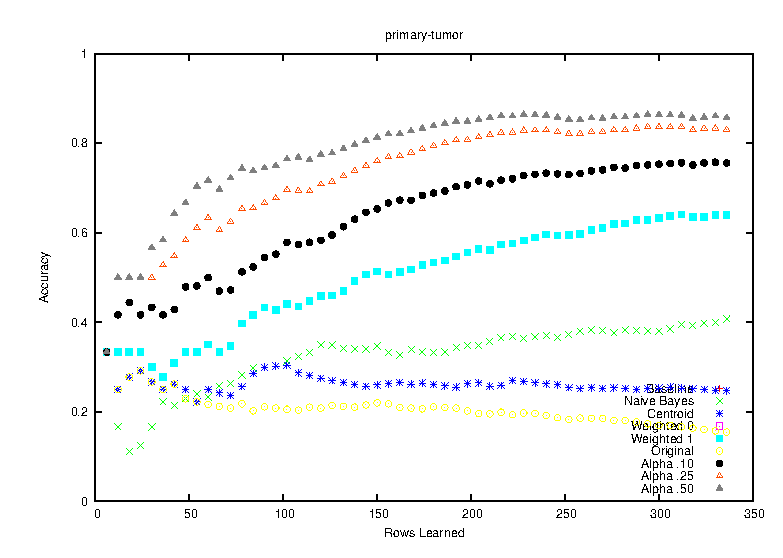
\epsfig{file=charts/primary-tumor.eps}
\caption{Incremental results from a discrete dataset with 22 class values}
\label{fig:primary-tumor}
\end{figure*}

\begin{figure*}
\centering
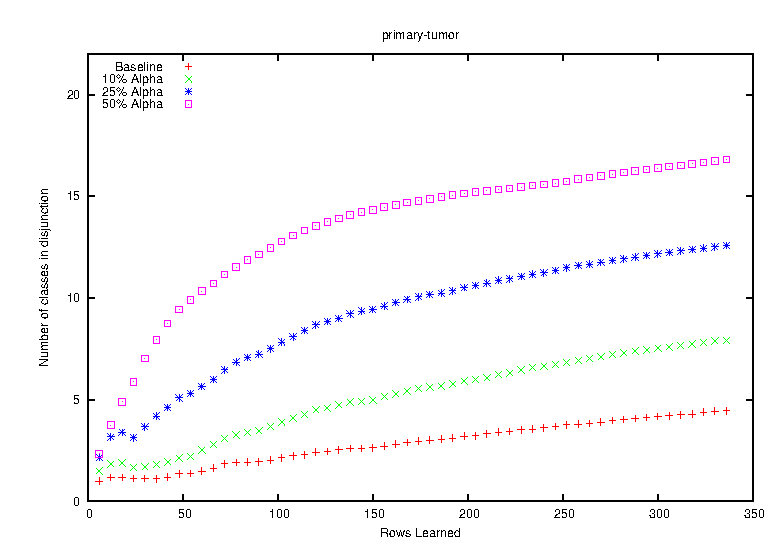
\epsfig{file=charts/primary-tumor-setsize.eps}
\caption{Average number of classes contained within disjunction for incremental learning}
\label{fig:primary-tumor-setsize}
\end{figure*}

\begin{figure*}
\centering
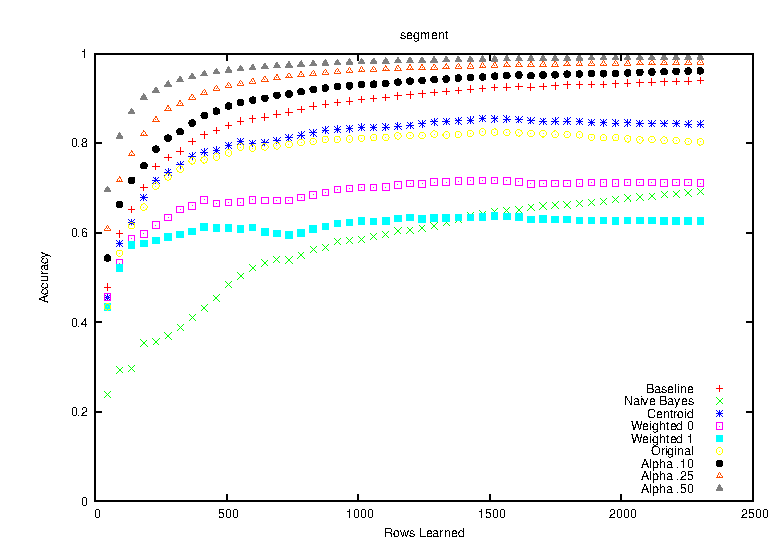
\epsfig{file=charts/segment.eps}
\caption{Incremental results from a numeric dataset with 7 discrete classes}
\label{fig:segment}
\end{figure*}

\begin{figure*}
\centering
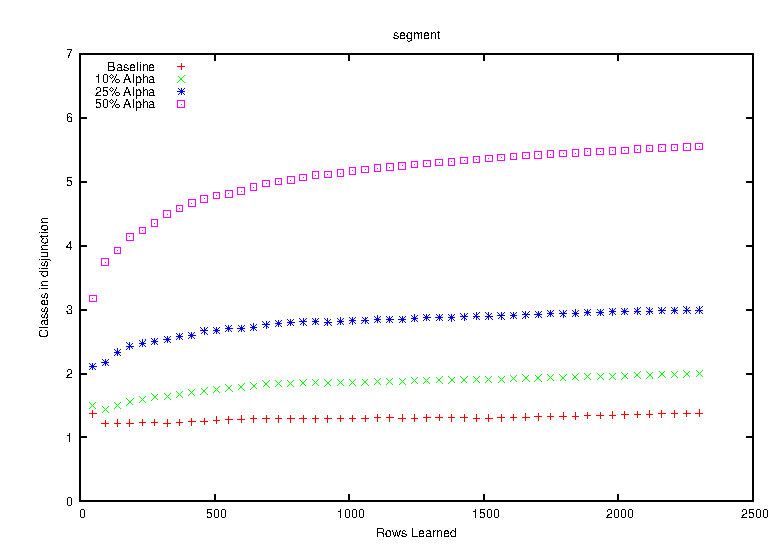
\epsfig{file=charts/segment-setsize.eps}
\caption{Average number of classes contained within disjunction for numeric attribute dataset}
\label{fig:segment-setsize}
\end{figure*}

Learning with disjoint sets introduces some caveats to data analysis. As seen in figure ~\ref{fig:primary-tumor}, our baseline disjunctive HyperPipes consistently outperforms both naive bayes and the original HyperPipes algorithm. However, our disjuntive learner doesn't exactly play fair, hedgings it's bets with multiple predicted classes. Note as well that when we use our centroid method for single classification, we fail to consistently beat naive bayes.

However, when disjunctive HyperPipes cheats, it does so with a conscious. Figure ~\ref{fig:primary-tumor-setsize} plots the average size of the sets returned for the primary-tumor dataset as we incrementally learn across the data. As our baseline results demonstrate, we return on average no more than 20\% of potential classes. As a result, we trade in single classification for a doubling of accuracy (figure ~\ref{fig:primary-tumor}).
